\documentclass[11pt,letterpaper]{article}
\pdfoutput=1
\usepackage{jheppub}
\usepackage{color}
\usepackage{graphicx}
\usepackage{tabularx}
\usepackage{xspace}

\usepackage{verbatim}
\usepackage{amsmath}
\usepackage{amssymb}
\usepackage[caption=false]{subfig}
\usepackage{url}
\usepackage{bbold}
\usepackage{slashed}
\usepackage{array}

\usepackage{multirow}
\usepackage{threeparttable}
\usepackage{paralist}


\newcommand{\GeV}{\text{GeV}}
\newcommand{\TeV}{\text{TeV}}
\newcommand{\SO}{\text{SO}}
\newcommand{\SU}{\text{SU}}
\newcommand{\SM}{\text{SM}}

\newcommand{\U}{\text{U}}
\newcommand{\CKM}{\text{CKM}}
\newcommand{\eff}{\text{eff}}

\newcommand{\ev}{\text{event}}
\newcommand{\jet}{\text{jet}}
\newcommand{\jets}{\text{jets}}
\newcommand{\subj}{\text{subjet}}
\newcommand{\subjs}{\text{subjets}}
\newcommand{\cut}{\text{cut}}
\newcommand{\trim}{\text{trim}}
\newcommand{\Ecut}{E_{{\rm cut}}}

\newcommand{\ptc}{p_{T{\rm cut}}}
\newcommand{\ptsubc}{p_{T{\rm subcut}}}

\newcommand{\sub}{\text{sub}}
\newcommand{\miss}{\text{miss}}

\newcommand{\pythia}{\textsc{Pythia~8}\xspace}
\newcommand{\herwig}{\textsc{Herwig++}\xspace}
\newcommand{\eventtwo}{\textsc{Event2}\xspace}

\newcommand{\FastJet}{\textsc{FastJet}\xspace}
\newcommand{\MadGraph}{\textsc{MadGraph}\xspace}

\newcommand{\df}{\text{d}}
\newcommand{\vev}[1]{\langle #1 \rangle}


\DeclareRobustCommand{\Sec}[1]{Sec.~\ref{#1}}
\DeclareRobustCommand{\Secs}[2]{Secs.~\ref{#1} and \ref{#2}}
\DeclareRobustCommand{\Secss}[3]{Secs.~\ref{#1}, \ref{#2}, and \ref{#3}}
\DeclareRobustCommand{\App}[1]{App.~\ref{#1}}
\DeclareRobustCommand{\Tab}[1]{Table~\ref{#1}}
\DeclareRobustCommand{\Tabs}[2]{Tables~\ref{#1} and \ref{#2}}
\DeclareRobustCommand{\Fig}[1]{Fig.~\ref{#1}}
\DeclareRobustCommand{\Figs}[2]{Figs.~\ref{#1} and \ref{#2}}
\DeclareRobustCommand{\Figss}[3]{Figs.~\ref{#1}, \ref{#2}, and \ref{#3}}
\DeclareRobustCommand{\Eq}[1]{Eq.~(\ref{#1})}
\DeclareRobustCommand{\Eqs}[2]{Eqs.~(\ref{#1}) and (\ref{#2})}
\DeclareRobustCommand{\Eqss}[3]{Eqs.~(\ref{#1}), (\ref{#2}), and (\ref{#3})}
\DeclareRobustCommand{\Ref}[1]{Ref.~\cite{#1}}
\DeclareRobustCommand{\Refs}[1]{Refs.~\cite{#1}}

\newcommand{\be}{\begin{equation}}
\newcommand{\ee}{\end{equation}}
\newcommand{\nn}{\nonumber}

\renewcommand{\textfraction}{0.10}
\renewcommand{\topfraction}{0.90}
\renewcommand{\bottomfraction}{0.90}
\renewcommand{\floatpagefraction}{0.65}

%% Reference commands %%
\newcommand{\mb}[1]{\boldsymbol{#1}}
\newcommand{\bm}[1]{\boldsymbol{#1}}
\newcommand{\mbo}[1]{\boldsymbol{\overline{#1}}}

\usepackage{xspace}


\def\Tr{\mathop{\rm Tr}}
\newcommand{\rep}[1]{\mathbf{#1}}
\newcommand{\conjrep}[1]{\overline{\mathbf{#1}}}


\renewcommand{\a}{\alpha}
\renewcommand{\b}{\beta}
\newcommand{\e}{\epsilon}
\newcommand{\D}{\Delta}
\renewcommand{\l}{\lambda}
\renewcommand{\th}{\theta}
\newcommand{\bq}{\bar{q}}
\newcommand{\zcut}{z_{\rm cut}}

\newcommand{\IZ}{\mathbb{Z}}
\newcommand{\cD}{\mathcal{D}}
\newcommand{\cL}{\mathcal{L}}
\newcommand{\cR}{\mathcal{R}}
\newcommand{\cF}{\mathcal{F}}
\newcommand{\cI}{\mathcal{I}}
\newcommand{\cK}{\mathcal{K}}
\newcommand{\beq}{\begin{eqnarray}}
\newcommand{\eeq}{\end{eqnarray}}

\newcommand{\F}{\mathcal{F}}
\newcommand{\Ft}{\widetilde{\mathcal{F}}}
\newcommand{\G}{\mathcal{G}}
\newcommand{\Gt}{\widetilde{\mathcal{G}}}
\newcommand{\HH}{\mathcal{H}}
\newcommand{\HHt}{\widetilde{\mathcal{H}}}
\newcommand{\ord}[1]{\mathcal{O}\!\left(#1\right)}

\newcommand*\numcircledmod[1]{#1 \!\!\! \bigcirc}

\newcommand{\Njet}{\widetilde{N}_{\rm jet}}
\newcommand{\dN}[1]{\Delta_{#1}}
\newcommand{\dNpm}{\Delta_{2\pm}}
\newcommand{\dNp}{\Delta_{2+}}
\newcommand{\dNm}{\Delta_{2-}}
\newcommand{\dNtm}{\Delta_{3-}}

\newcommand{\cT}{\mathcal{T}}
\newcommand{\as}{\alpha_s}
\renewcommand{\angle}{\theta}

\definecolor{darkgreen}{rgb}{0,0.5,0}
\newcommand{\jdt}[1]{\textbf{\textcolor{darkgreen}{(#1 --jdt)}}}


\begin{document}


\title{Systematics of Quark/Gluon Tagging}

\author{Samuel Bein,}
\emailAdd{samuel.bein@gmail.com}
\author{Andy Buckley,}
\emailAdd{andy.buckley@cern.ch}
\author{Mario Campanelli,}
\emailAdd{mario.campanelli@cern.ch}
\author{Marat Freytsis,}
\emailAdd{freytsis@physics.harvard.edu}
\author{Philippe Gras,}
\emailAdd{philippe.gras@cern.ch}
\author{\\Deepak Kar,}
\emailAdd{deepak.kar@cern.ch}
\author{Simon Pl\"atzer,}
\emailAdd{simon.plaetzer@desy.de}
\author{Chris Pollard,}
\emailAdd{cspollard@gmail.com}
\author{Salvatore Rappoccio,}
\emailAdd{rappoccio@gmail.com}
\author{Andrzej Siodmok,}
\emailAdd{andrzej@cern.ch}
\author{Peter Skands,}
\emailAdd{peter.skands@monash.edu}
\author{Dave Soper,}
\emailAdd{soper@uoregon.edu}
\author{Gregory Soyez,}
\emailAdd{soyez@lpthe.jussieu.fr}
\author{Frank Tackmann,}
\emailAdd{frank.tackmann@desy.de}
\author[a]{Jesse Thaler}
\affiliation[a]{Center for Theoretical Physics, Massachusetts Institute of Technology, \\ Cambridge, MA 02139, U.S.A.}
\emailAdd{jthaler@mit.edu}

%\date{\today}

\abstract{\jdt{Author list is going to contract.  This abstract is aspirational at the moment.}  By measuring the substructure of a jet, one can assign it a ``quark'' or ``gluon'' tag.  In the eikonal limit, quark/gluon discrimination is determined solely by the color factor of the initiating parton ($C_F$ versus $C_A$).  The goal of this paper is to go beyond this leading order understanding, using both parton shower generators and first-principles calculations to assess the impact of higher-order perturbative and non-perturbative physics.  In the idealized context of electron-positron collisions, where there exists an unambiguous definition of quark and gluon jets, we find a fascinating interplay between perturbative shower effects and non-perturbative hadronization effects.  Turning to proton-proton collisions, we highlight a core set of measurements which would constrain the leading uncertainties in quark/gluon tagging and improve the overall modeling of jets at the Large Hadron Collider.}

\preprint{MIT--CTP xxxx}

\maketitle

%-----------------------------------------------------------
\section{Introduction}
\label{introduction}

Jets are a robust tool for studying short-distance collisions involving quarks and gluons.  With a suitable jet definition, one can connect jet measurements made on clusters of hadrons to perturbative calculations made on clusters of partons \cite{}.  More ambitiously, one can try to tag jets with a suitably-defined flavor label, thereby enhancing the fraction of, say, quark-tagged jets over gluon-tagged jets.  This is relevant for searches for physics beyond the standard model, where signals of interest are often dominated by quarks while the corresponding backgrounds are dominated by gluons.  A wide variety of quark/gluon discriminants have been proposed \cite{}, and there is a growing catalog of quark/gluon studies at the Large Hadron Collider (LHC) \cite{}.

In order to achieve robust quark/gluon tagging, though, one needs theoretical and experimental control over quark/gluon radiation patterns.  At the level of eikonal partons, a quark radiates proportional to its $C_F = 4/3$ color factor while a gluon radiates proportional to $C_A = 3$.  In this paper, we will demonstrate that quark/gluon discrimination performance is highly sensitive to subleading perturbative effects beyond the eikonal limit, such as $g \to q \overline{q}$ splittings and color coherence, as well as to non-perturbative effects such as color reconnection and hadronization.   While these effects are modeled (to differing degrees) in parton shower generators, they are relatively unconstrained by existing collider measurements, especially in the gluon channel.  The goal of this paper is to highlight these uncertainties and suggest a set of future LHC measurements that will improve the modeling of jets in general and quark/gluon tagging in particular.

A common misconception about quark/gluon tagging is that it is somehow an intrinsically ill-defined problem.  Of course, quark and gluon partons carry color while jets are composed of color-singlet hadrons, so the labels ``quark'' and ``gluon'' are intrinsically ambiguous.  But this is philosophically no different from the fact that a ``jet'' is intrinsically ambiguous and one must therefore always specify a concrete jet finding procedure.  As discussed in \Sec{sec:quarkgluondef}, we can think about quark/gluon discrimination in the context of unambiguous hadron-level measurements.  In this sense, quark/gluon tagging is a well-defined technique for enhancing desired signals over undesired backgrounds.

There are a wide range of possible quark/gluon discriminants and a similarly large range of ways to quantify discrimination power, discussed further in  \Sec{sec:prelim}.  As a concrete set of discriminants, we consider the generalized angularities $\lambda_\beta^\kappa$ \cite{} at five different $(\kappa, \beta)$ working points.  These roughly map onto five variables in common use in the literature:
\be
\text{multiplicity}, \quad p_T^D, \quad \text{LHA}, \quad \text{width}, \quad \text{mass},
\ee
where LHA refers to the ``Les Houches Angularity'', named after the workshop where this study was initiated.  To quantify discrimination performance, we focus on classifier separation \cite{}:
\be
\Delta =  \frac{1}{2} \int \df \lambda \, \frac{\bigl(p_q(\lambda) - p_g(\lambda)\bigr)^2}{p_q(\lambda) + p_g(\lambda)},
\ee
where $p_q$ ($p_g$) is the probability distribution for a pure quark (gluon) sample,  though we also show some results in terms of ROC curves.

To avoid some of the complications in properly defining quark and gluon samples, we start our study in \Sec{sec:ee} by comparing the jets produced in the following processes:
\begin{align}
\text{``quark jets''}: \quad & e^+e^- \to (\gamma/Z)^* \to u \overline{u}, \\
\text{``gluon jets''}: \quad & e^+e^- \to h^* \to g g.
\end{align}
These processes are physically distinguishable by the quantum numbers of the associated color singlet production operator, giving a way to label quarks and gluons without reference to the final state.  We compare four different Monte Carlo generators, not only at their default configurations but also with physically-motivated changes.
\begin{itemize}
\item \textsc{Pythia 8.205} \cite{}
\item \textsc{Vincia 1.201} \cite{}
\item \textsc{Herwig++ 2.7.1} \cite{}
\item \textsc{Sherpa 2.1.1} \cite{}
\end{itemize}
As we will see, the dominant differences between programs arise from physics at the interface between perturbative showering and non-perturbative fragmentation.  We verify some of the observed behavior in the generators with analytic resummed calculations.

Turning to the LHC in \Sec{sec:pp}, we










\section{What is a Quark/Gluon Jet?}
\label{sec:quarkgluondef}


\section{Preliminaries}
\label{sec:prelim}

\subsection{Generalized Angularities}

\subsection{Metrics for Discrimination Power}

For our studies, we need a way to quantify quark/gluon separation power in a robust way that does not require enormous Monte Carlo data sets.

The standard way to quantify discrimination power is through ROC curves.  At a point ($q$,$g$) on the ROC curve, where $q,g \in [0,1]$, one can define a selection that yields $q$ efficiency for quarks and $g$ mistag rate for gluons, or equivalently, a $(1-g)$ efficiency for gluons for a $(1-q)$ mistag rate for quarks.  From the ROC curve, we define five benchmark points, visualized in \Fig{fig:roc_curve}:
\begin{align}
\{ g^{\rm  rej}_{50} ,   g^{\rm  rej}_{20}\} : \quad & \text{Gluon rejection rate at \{50\%, 20\%\} quark efficiency}; \\
\{q^{\rm rej}_{50} ,  q^{\rm rej}_{20}\} : \quad & \text{Quark rejection rate at \{50\%, 20\%\} gluon efficiency}; \\
s^{\rm rej} : \quad & \text{Symmetric rejection rate at $s^{\rm rej}$ efficiency}.
\end{align}
For all of these measures, $x^{\rm rej} \in [\frac{1}{2},1]$, where $\frac{1}{2}$ corresponds to no discrimination and $1$ corresponds to optimal discrimination.  To assign statistical errors to these quantities in Monte Carlo, we make the simplifying assumption that the uncertainty is only due to Poisson statistics on the $x^{\rm rej}$ value.

\begin{figure}
\centering
\subfloat{
\label{fig:roc_curve}
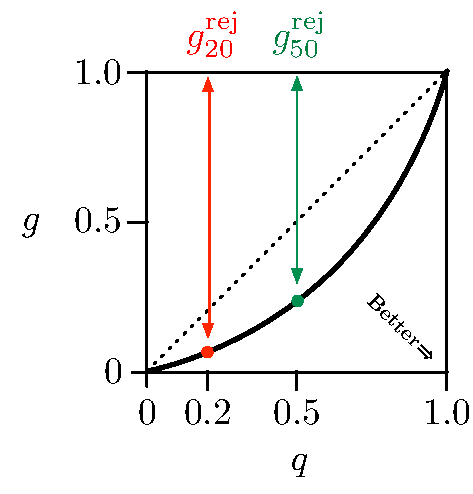
\includegraphics[scale = 0.85]{figures/roc_curve}
}
$\quad$
\subfloat{
\label{fig:truth_overlap}
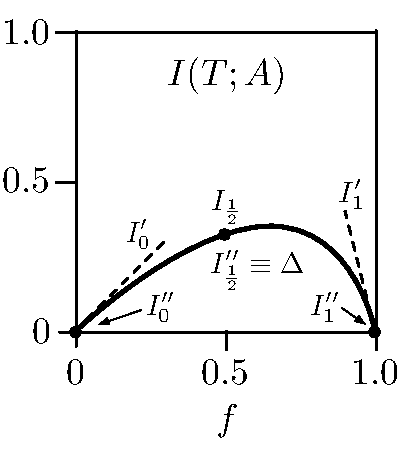
\includegraphics[scale = 0.85]{figures/truth_overlap}
}
\caption{(a) Five ROC Curve benchmark points.  (b) Six mutual information benchmark values.}
\end{figure}

An alternative way to quantify discrimination power is through mutual information, which counts the number of ``bits'' of information gained from measuring a discriminant variable (see \cite{Larkoski:2014pca}).  Given a sample with quark fraction $f \in [0,1]$ and gluon fraction $(1-f)$, the mutual information with the truth (a.k.a. the truth overlap) is:
\be
I(T;A) = \int \df a \left(f \, p_q(a) \log_2 \frac{p_q(a)}{p_{\rm tot}(a)} + (1-f) \, p_g(a) \log_2 \frac{p_g(a)}{p_{\rm tot}(a)}   \right),
\ee
where $p_q$ ($p_g$) is the probability distribution for quarks (gluons), and
\be
p_{\rm tot}(a) = f \, p_q(a) + (1-f) \, p_g(a).
\ee
The minimum value of $I(T;A)$ is $0$ (no discrimination) and the maximum value is
\be
I(T;A)_{\rm max} = f \log_2 \frac{1}{f} + (1-f) \log_2 \frac{1}{1-f},
\ee
which equals $1$ for $f = \frac{1}{2}$.

The choice $f = 1/2$ was used in \Ref{Larkoski:2014pca}, $I(T;A)\big|_{f = \frac{1}{2}} \equiv I_{\frac{1}{2}}$, though other $f$ choices are plausible.  The first derivative at $f = 1/2$ is not particularly enlightening, but the second derivative is sometimes referred to as the classifier separation:
\be
- \frac{\log 2}{4} \frac{\partial^2 I(T;A)}{\partial f^2} \Big|_{f = \frac{1}{2}} \equiv I''_\frac{1}{2} = \frac{1}{2} \int \df a \, \frac{\left(p_q(a) - p_g(a)\right)^2}{p_q(a) + p_g(a)},
\ee
where the normalization has been set such that $I''_\frac{1}{2} \in [0,1]$.  At $f = 0$ and $f = 1$, the mutual information itself is zero, but the derivatives are related to other concepts in statistics:
\be
\frac{\partial I}{\partial f} \Big|_{f = 0} \equiv I'_0 = \int \df a \, p_q(a)  \log_2 \frac{p_q(a)}{p_g(a)}, \qquad - \log 2 \,  \frac{\partial^2 I}{\partial f^2} \Big|_{f = 0} \equiv I''_0 = \int \df a \,  \frac{p_q(a)^2}{p_g(a)},
\ee
\be
- \frac{\partial I}{\partial f} \Big|_{f = 1} \equiv I'_1 = \int \df a \, p_g(a) \log_2 \frac{p_g(a)}{p_q(a)}, \qquad - \log 2 \, \frac{\partial^2 I}{\partial f^2} \Big|_{f = 1} \equiv I''_1 = \int \df a \, \frac{p_g(a)^2}{p_q(a)}.
\ee
The first derivative is sometimes called relative entropy and the second derivative is sometimes called discrimination significance.  However, all of these quantities become singular if the probability distribution is zero, so we will only quote the values at $f = \frac{1}{2}$, visualized in \Fig{fig:truth_overlap}:
\be
\{I_\frac{1}{2}, I''_{\frac{1}{2}} \}.
\ee
To assign statistical errors to these quantities in Monte Carlo, we evaluate $I(T;A)$ in bins of $a$ and use Poisson statistics.  Note that there is a binning bias in $I_\frac{1}{2}$, so we use the method explained in Appendix A.3 of \Ref{Larkoski:2014pca} and use half the $\Delta a$ bin size on the combined quark/gluon sample compared to the individual quark/gluon samples.

\subsection{Parton-level Quark/Gluon Tags}

\section{Idealized Quark/Gluon Tagging}
\label{sec:ee}

\subsection{Parton-Level Performance}

\subsection{Hadron-Level Performance}

\subsection{Predictions from Resummation}

\section{Quark/Gluon Tagging at the LHC}
\label{sec:pp}

\subsection{Enriched Quark/Gluon Samples}

\subsection{Tagging Performance}


\section{Conclusions}




\begin{acknowledgments}
We thank Jon Butterworth, Peter Loch, Alexander Schmidt

\end{acknowledgments}


\bibliographystyle{JHEP}
\bibliography{lh2015_qg}

\end{document}
